\section{Cross-Era Synthesis}
\label{sec:synthesis}

\begin{figure*}[t]
  \centering
  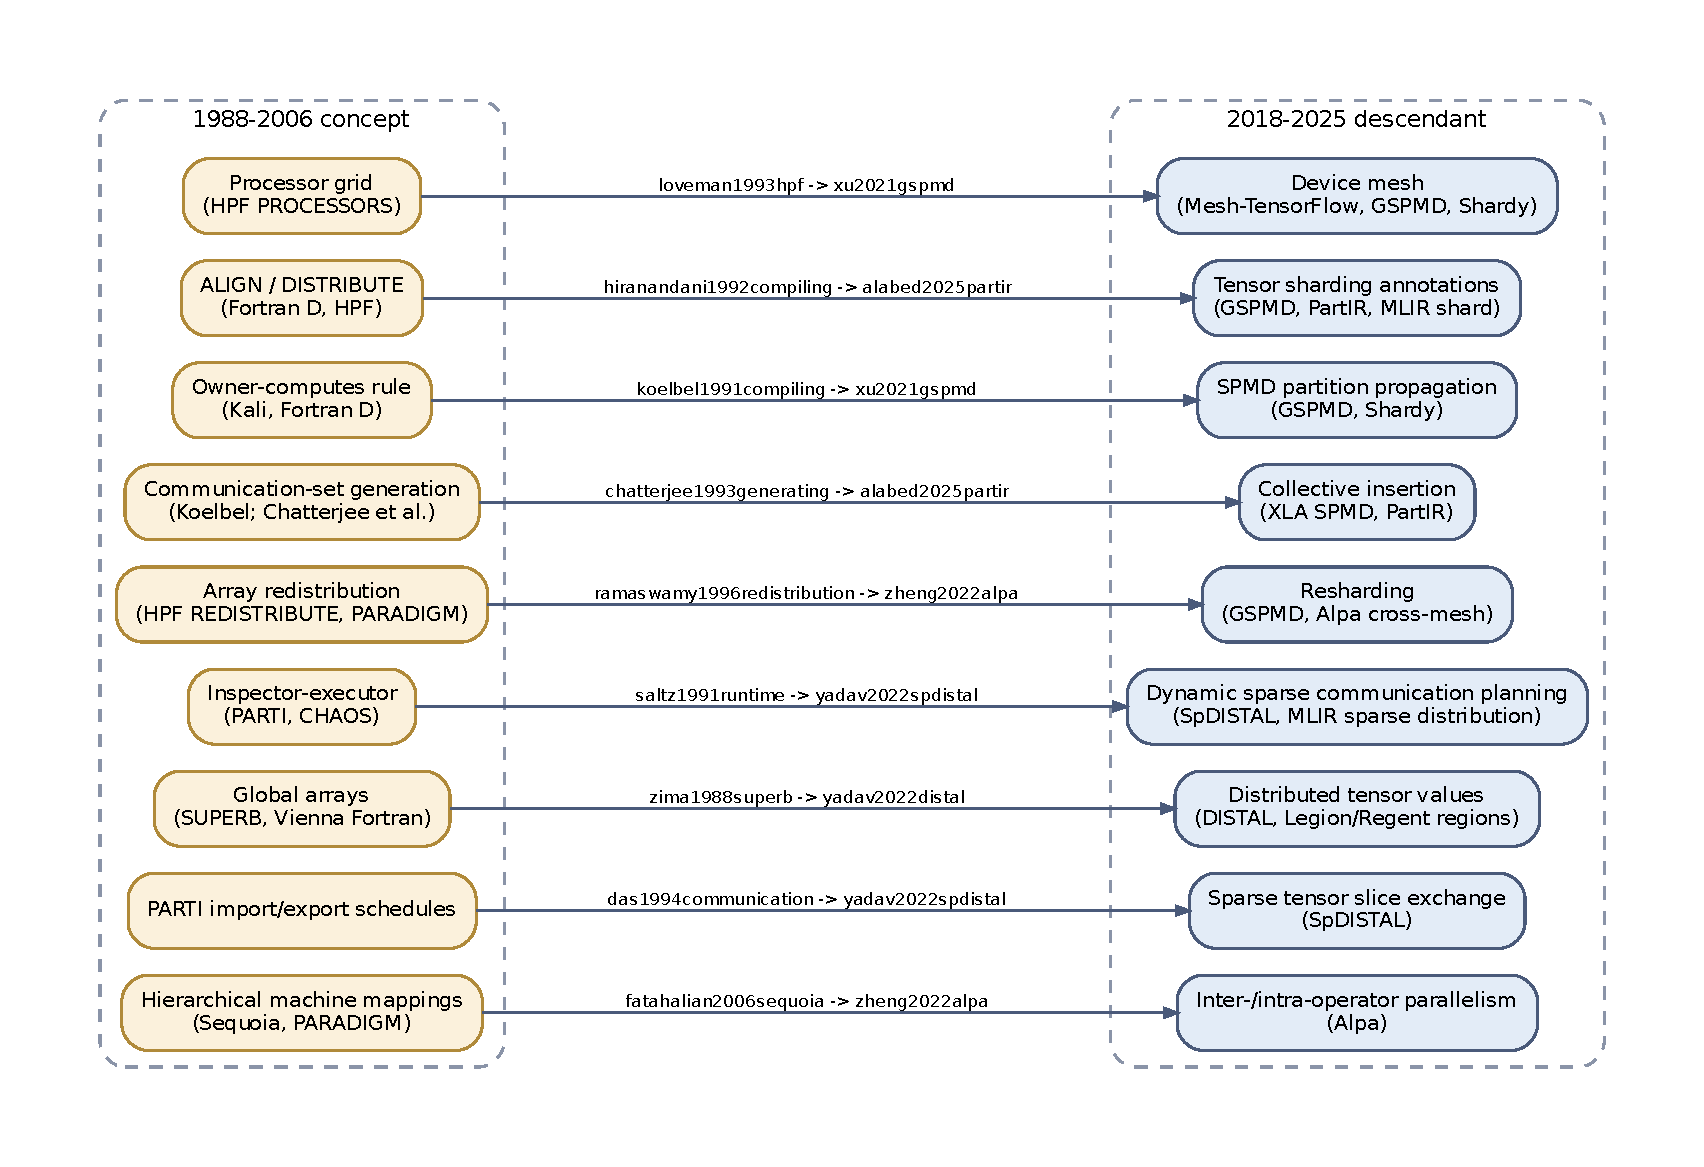
\includegraphics[width=0.9\textwidth]{rediscovery-map.pdf}
  \caption{Concepts of 1988--2006 and their 2018--2025 descendants. Each edge names the catalog entries that document the older and the newer form. The pairing is a survey hypothesis: it asserts functional correspondence, not that the newer work cites the older one; evidence for each pair is tracked in the repository's historical-claims file.}
  \label{fig:rediscovery}
\end{figure*}

\subsection{Ideas that persisted}
\infer{Logical processor grids, block distributions, owner-derived computation mapping, and the separation of a global index space from local storage persisted from Era~2 through Era~6 (Fig.~\ref{fig:rediscovery}).}

\subsection{Ideas that failed or receded}
\infer{Fully automatic distribution selection for general Fortran programs receded after Era~3; the HPF retrospective attributes HPF's decline to immature compilers, unpredictable performance, and missing support for irregular codes~\cite{kennedy2007rise}.} \todo{Confirm the attribution against the text of \cite{kennedy2007rise} and \cite{benkner1999compiling}.}

\subsection{Concepts rediscovered under new names}
\infer{Processor grid $\rightarrow$ device mesh; ALIGN/DISTRIBUTE $\rightarrow$ sharding annotation; owner-computes $\rightarrow$ partition propagation; communication sets $\rightarrow$ collective insertion; redistribution $\rightarrow$ resharding; inspector--executor $\rightarrow$ dynamic sparse communication planning; global arrays $\rightarrow$ distributed tensor values; PARTI import/export $\rightarrow$ sparse slice exchange; hierarchical machine mapping $\rightarrow$ inter-/intra-operator parallelism.}

\subsection{Why explicit MPI became dominant, and why high-level partitioning has returned}
\infer{We hypothesise that MPI won in Era~3--4 because its cost model is transparent to the programmer and its performance does not depend on compiler maturity, whereas high-level partitioning has returned in Era~6 because ML programs are expressed as operator graphs with few, large, regular operators, which makes both propagation and cost modelling tractable in a way that general Fortran loops were not.} \todo{Test this hypothesis against the evaluation sections of \cite{xu2021gspmd,zheng2022alpa,alabed2025partir} and against \cite{kennedy2007rise}.}
